\documentclass[10 pt, titlepage]{article}\usepackage[]{graphicx}\usepackage[]{color}
%% maxwidth is the original width if it is less than linewidth
%% otherwise use linewidth (to make sure the graphics do not exceed the margin)
\makeatletter
\def\maxwidth{ %
  \ifdim\Gin@nat@width>\linewidth
    \linewidth
  \else
    \Gin@nat@width
  \fi
}
\makeatother

\definecolor{fgcolor}{rgb}{0.345, 0.345, 0.345}
\newcommand{\hlnum}[1]{\textcolor[rgb]{0.686,0.059,0.569}{#1}}%
\newcommand{\hlstr}[1]{\textcolor[rgb]{0.192,0.494,0.8}{#1}}%
\newcommand{\hlcom}[1]{\textcolor[rgb]{0.678,0.584,0.686}{\textit{#1}}}%
\newcommand{\hlopt}[1]{\textcolor[rgb]{0,0,0}{#1}}%
\newcommand{\hlstd}[1]{\textcolor[rgb]{0.345,0.345,0.345}{#1}}%
\newcommand{\hlkwa}[1]{\textcolor[rgb]{0.161,0.373,0.58}{\textbf{#1}}}%
\newcommand{\hlkwb}[1]{\textcolor[rgb]{0.69,0.353,0.396}{#1}}%
\newcommand{\hlkwc}[1]{\textcolor[rgb]{0.333,0.667,0.333}{#1}}%
\newcommand{\hlkwd}[1]{\textcolor[rgb]{0.737,0.353,0.396}{\textbf{#1}}}%

\usepackage{framed}
\makeatletter
\newenvironment{kframe}{%
 \def\at@end@of@kframe{}%
 \ifinner\ifhmode%
  \def\at@end@of@kframe{\end{minipage}}%
  \begin{minipage}{\columnwidth}%
 \fi\fi%
 \def\FrameCommand##1{\hskip\@totalleftmargin \hskip-\fboxsep
 \colorbox{shadecolor}{##1}\hskip-\fboxsep
     % There is no \\@totalrightmargin, so:
     \hskip-\linewidth \hskip-\@totalleftmargin \hskip\columnwidth}%
 \MakeFramed {\advance\hsize-\width
   \@totalleftmargin\z@ \linewidth\hsize
   \@setminipage}}%
 {\par\unskip\endMakeFramed%
 \at@end@of@kframe}
\makeatother

\definecolor{shadecolor}{rgb}{.97, .97, .97}
\definecolor{messagecolor}{rgb}{0, 0, 0}
\definecolor{warningcolor}{rgb}{1, 0, 1}
\definecolor{errorcolor}{rgb}{1, 0, 0}
\newenvironment{knitrout}{}{} % an empty environment to be redefined in TeX

\usepackage{alltt}
\usepackage[left=1in, right=.75in,top=.5in,bottom=.65in]{geometry}
\usepackage{color, xcolor}

\usepackage{tikz}
\usetikzlibrary{intersections}

\usetikzlibrary{positioning, shapes}

\definecolor{light-gray}{gray}{0.95}
\definecolor{drkgreen}{RGB}{5,102,51}
\IfFileExists{upquote.sty}{\usepackage{upquote}}{}


\begin{document}

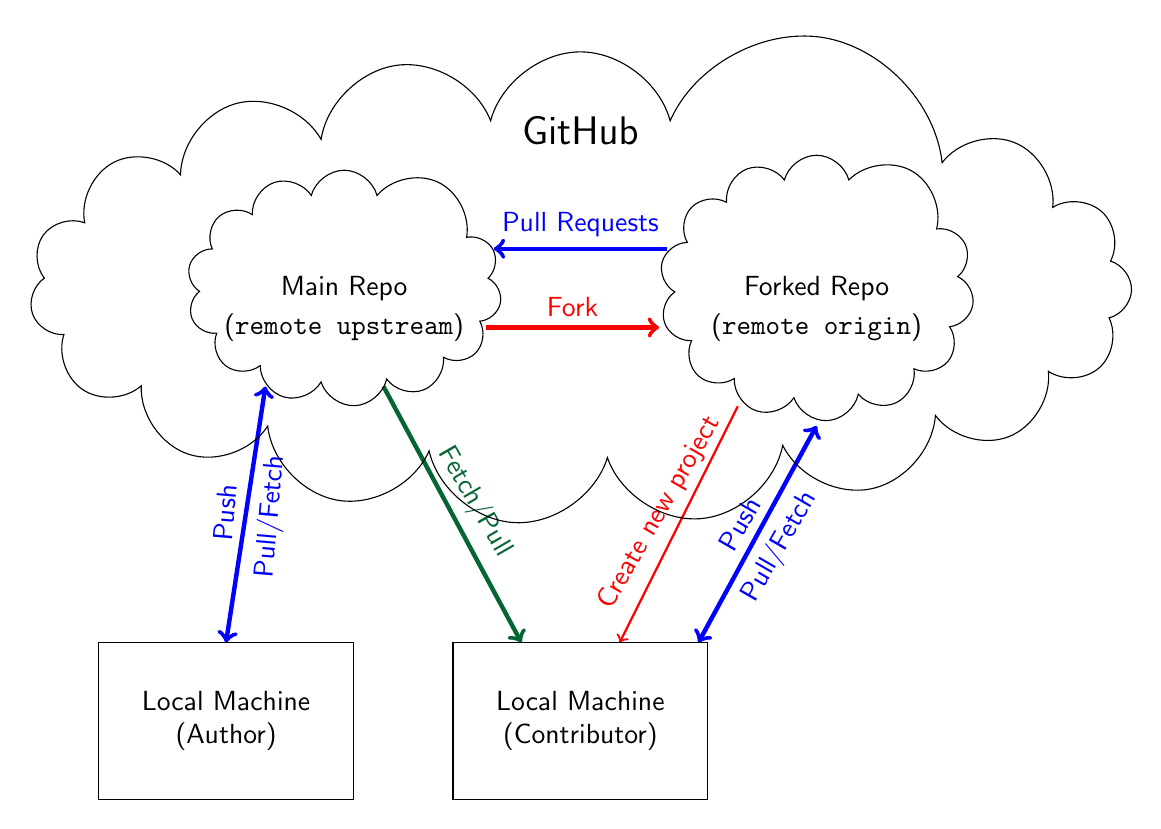
\begin{tikzpicture}\sffamily
  \coordinate (main) at (1.9,.5);
  \coordinate (main2) at (1.8,-.5);
  \coordinate(main3) at (-1,-1.25);
  \coordinate (fork) at (4.1,.5);
  \coordinate (fork2) at (4,-.5);
  \coordinate (fork3) at (5,-1.5);
  \coordinate (fork4) at (6.,-1.75);
  \coordinate (loc) at (3,-5.5);
  \coordinate(loc1) at (3.5,-4.5);
  \coordinate (loc2) at (2.25,-4.5);
  \coordinate (loc3) at (4.5,-4.5);
  \coordinate (auth) at (-1.5,-5.5);
  \coordinate (auth1) at (-1.5,-4.5);
  \path[<-, blue, draw, ultra thick, name path= path1] (main) -- node[above]{Pull Requests} (fork) ;
  \path[ ->, red, draw,ultra thick, name path= path2] (main2) --node[above]{Fork} (fork2);
  
  \path[ ->, drkgreen, draw, ultra thick, name path= path3] 
            (0.5,-1.25) --node[above, rotate=300]{Fetch/Pull} (loc2);
            
  \path[ <-, draw, red, thick, name path= path4] (loc1) -- node[above, rotate=60]{Create new project}(fork3);
  \path[ <->,blue, draw, ultra thick, name path= path5] 
          (loc3) -- node[above, rotate=60]{Push} node[below, rotate=60]{Pull/Fetch} (fork4);
 \path[ <->,blue, draw, ultra thick, name path= path6] 
          (auth1) -- node[above, rotate=85]{Push} node[below, rotate=85]{Pull/Fetch} (main3);
    \node[
        name path=mainrepo,
        cloud, cloud puffs=13.7,
        minimum width=4cm,minimum height=2.5cm, draw,
    ] (mainrepo) at (0,0) {Main Repo};
    \node at (0,-.5) {(\texttt{remote upstream})};
    \node[
        cloud, cloud puffs=13.7,
        minimum width=4cm, minimum height=2.5cm, draw,
    ] (forked) at (6,0) {Forked Repo};
    \node at (6,-.5) {(\texttt{remote origin})};
     \node[cloud, cloud puffs=18.7,
        minimum width=14cm,minimum height=6cm, draw,
    ] (git) at (3,0) {};
    \node at (3,2) {\Large{GitHub}};
    \node[rectangle,
        minimum width=3cm,text width=3cm,align=center, minimum height=2cm, draw,
    ] (local) at (loc) {Local Machine (Contributor)};
    
   \node[rectangle,
        minimum width=3cm,text width=3cm,align=center, minimum height=2cm, draw,
    ] (author) at (auth) {Local Machine\quad (Author)};
   
\end{tikzpicture}
\end{document}


